\documentclass[letter,10pt]{article}
\usepackage[utf8]{inputenc}
\usepackage[english]{babel}
\usepackage{fancyvrb}
\usepackage{fancyhdr}
\usepackage{url}
\usepackage{verbatim}
\usepackage{graphicx}
\usepackage{rotating}
\usepackage{listings}
\usepackage{float}


\lstset{
language=C
}

\parskip 1mm
\setlength{\topmargin}{0pt}
\oddsidemargin  0.5cm
\evensidemargin 0.5cm
\textwidth      15.5cm
\textheight     21.0cm
\headsep        4 mm
\parindent      0.5cm

\pagestyle{fancyplain}

\lhead{Estadística Computacional 2015}
\rhead{\bf \it LEC 1 }
\lfoot{}
\cfoot{}
\rfoot{\bf \thepage}
\renewcommand{\footrulewidth}{0.4pt}

\title{LEC1 \\ Estadística Computacional 2015-1, UTFSM }
\author{Gonzalo Moya 201173016-k}

\date{\vspace*{1cm} Valparaíso, 29 de Noviembre del 2015}

\newpage

\begin{document}
\maketitle
\thispagestyle{empty}
\newpage
\tableofcontents

\makeatother

\newpage

\section{Introducción}

Este infrome aborda distintos problemas de probabilidad basándose en la noción frecuentista de esta con el fin de analizar
el cómo la simulación de experimentos nos permite relacionar la probabilidad empírica con la probabilidad teórica, demostrando como la
primera converge a la segunda y por tanto probando que la simulación es un método correcto para estudiar probabilidades.


\section{Desarrollo}
\subsection{Pregunta 1}
El problema en cuestión es el famoso Monty Hall Problem para un caso particular de 5 puertas.
\begin{itemize}
 \item[a)] El jugador en cuestión inicialmente tenía la probabilidad de $\frac{1}{5}$ de acertar a la puerta, una vez que el presentador
 abre una puerta y a su vez el participante decide cambiar de elección entonces las otras 3 puertas restantes tienen 
 \item[b)]
 \item[c)]
\end{itemize}

\subsection{Pregunta 2}
?
\subsection{Pregunta 3}
?
\subsection{Pregunta 4}
\begin{itemize}
 \item[a)] Para responder a la pregunta se realizan distintos experimentos para $n= 100,500,1000,1500$, A continuación se muestra el para $n=100$.
    0    1    2    3    4    5    6    7 
0.03 0.10 0.32 0.60 0.88 0.98 0.99 1.00 

 p real
[1] 0.01822838 0.10800994 0.30700341 0.56836796 0.79364860 0.92679954 0.98145105
[8] 0.99683271

suma [1] 0.2156783
  \begin{minipage}{\linewidth}
      \centering
      \begin{minipage}{0.45\linewidth}
          \begin{figure}[H]
              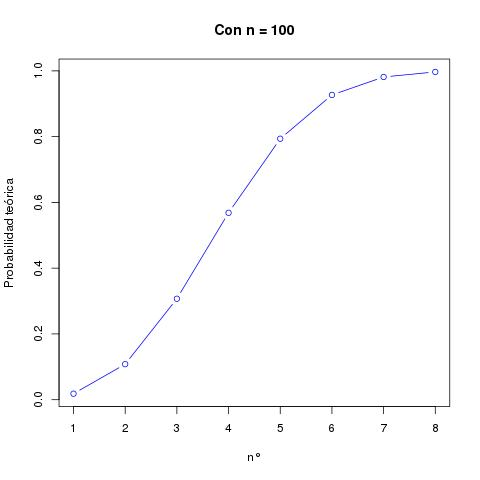
\includegraphics[width=\linewidth]{p3_teo_100.jpg}
              \caption{P. Te\'orica para n = 100}
          \end{figure}
      \end{minipage}
      \hspace{0.05\linewidth}
      \begin{minipage}{0.45\linewidth}
          \begin{figure}[H]
              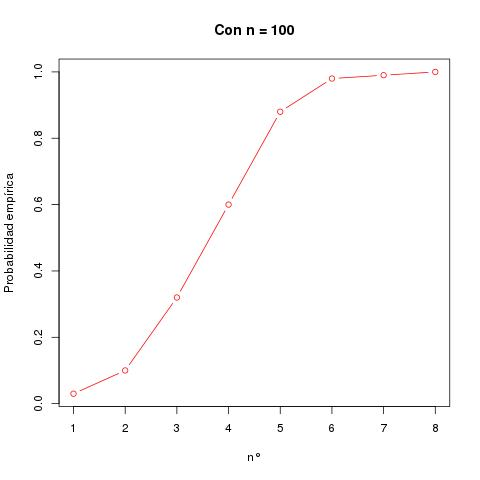
\includegraphics[width=\linewidth]{p3_emp_100.jpg}
              \caption{P. Emp\'irica para n = 100}
          \end{figure}
      \end{minipage}
  \end{minipage}


Para n = 500

frec acum
    0     1     2     3     4     5     6     7     8 
0.024 0.116 0.304 0.552 0.756 0.934 0.984 0.992 1.000


[1] 0.01822838 0.10800994 0.30700341 0.56836796 0.79364860 0.92679954 0.98145105
[8] 0.99683271 0.99967373

[1] 0.08569003


  \begin{minipage}{\linewidth}
      \centering
      \begin{minipage}{0.45\linewidth}
          \begin{figure}[H]
              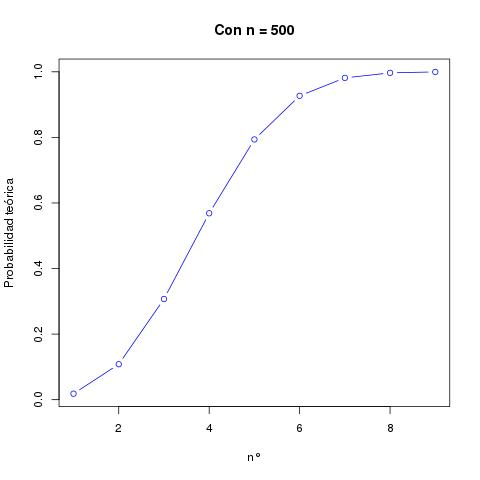
\includegraphics[width=\linewidth]{p4_teo_500.jpg}
              \caption{P. Te\'orica para n = 500}
          \end{figure}
      \end{minipage}
      \hspace{0.05\linewidth}
      \begin{minipage}{0.45\linewidth}
          \begin{figure}[H]
              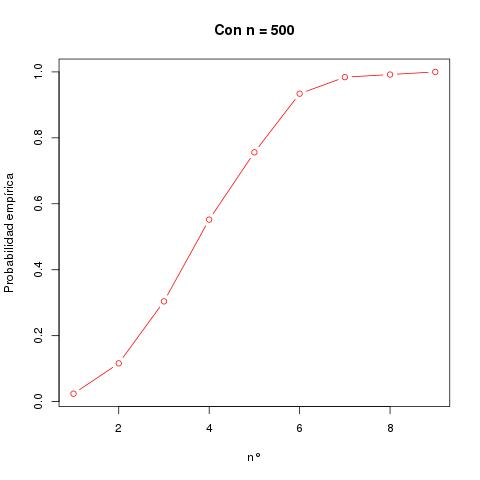
\includegraphics[width=\linewidth]{p4_emp_500.jpg}
              \caption{P. Emp\'irica para n = 500}
          \end{figure}
      \end{minipage}
  \end{minipage}
  
 frec acum
    0     1     2     3     4     5     6     7     8     9 
0.033 0.127 0.318 0.583 0.804 0.938 0.982 0.996 0.998 1.000 
 p real
 [1] 0.01822838 0.10800994 0.30700341 0.56836796 0.79364860 0.92679954 0.98145105
 [8] 0.99683271 0.99967373 0.99998468
 suma
[1] 0.08401288

  \begin{minipage}{\linewidth}
      \centering
      \begin{minipage}{0.45\linewidth}
          \begin{figure}[H]
              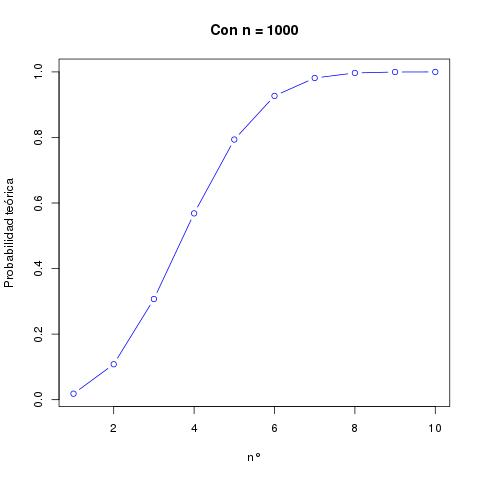
\includegraphics[width=\linewidth]{p4_teo_1000.jpg}
              \caption{P. Te\'orica para n = 1000}
          \end{figure}
      \end{minipage}
      \hspace{0.05\linewidth}
      \begin{minipage}{0.45\linewidth}
          \begin{figure}[H]
              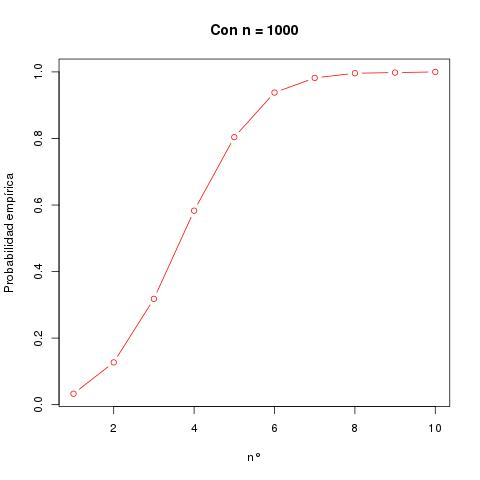
\includegraphics[width=\linewidth]{p4_emp_1000.jpg}
              \caption{P. Emp\'irica para n = 1000}
          \end{figure}
      \end{minipage}
  \end{minipage}
  
  
  
  
 frec acum
         0          1          2          3          4          5          6 
0.02133333 0.11333333 0.30800000 0.56066667 0.79533333 0.92000000 0.97800000 
         7          8 
0.99600000 1.00000000 
p real
[1] 0.01822838 0.10800994 0.30700341 0.56836796 0.79364860 0.92679954 0.98145105
[8] 0.99683271 0.99967373
suma
[1] 0.03022055
 
  \begin{minipage}{\linewidth}
      \centering
      \begin{minipage}{0.45\linewidth}
          \begin{figure}[H]
              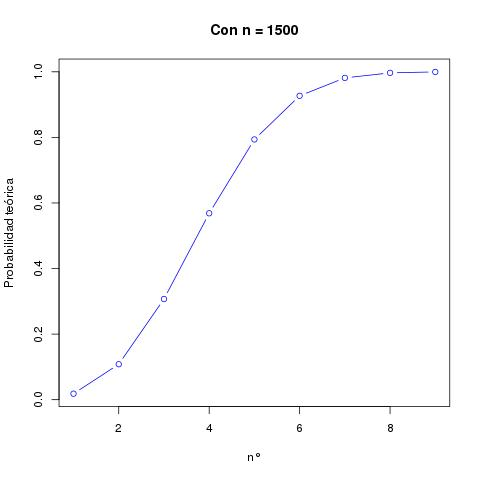
\includegraphics[width=\linewidth]{p4_teo_1500.jpg}
              \caption{P. Te\'orica para n = 1500}
          \end{figure}
      \end{minipage}
      \hspace{0.05\linewidth}
      \begin{minipage}{0.45\linewidth}
          \begin{figure}[H]
              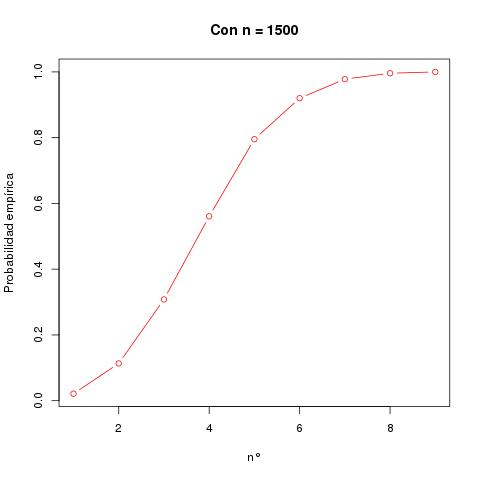
\includegraphics[width=\linewidth]{p4_emp_1500.jpg}
              \caption{P. Emp\'irica para n = 1500}
          \end{figure}
      \end{minipage}
  \end{minipage}

  
frec acum
      0       1       2       3       4       5       6       7       8       9 
0.01827 0.10744 0.30679 0.57137 0.79618 0.92856 0.98189 0.99710 0.99967 1.00000 
 p real
 [1] 0.01822838 0.10800994 0.30700341 0.56836796 0.79364860 0.92679954 0.98145105
 [8] 0.99683271 0.99967373 0.99998468
 suma
[1] 0.008844152
 
 
  \begin{minipage}{\linewidth}
      \centering
      \begin{minipage}{0.45\linewidth}
          \begin{figure}[H]
              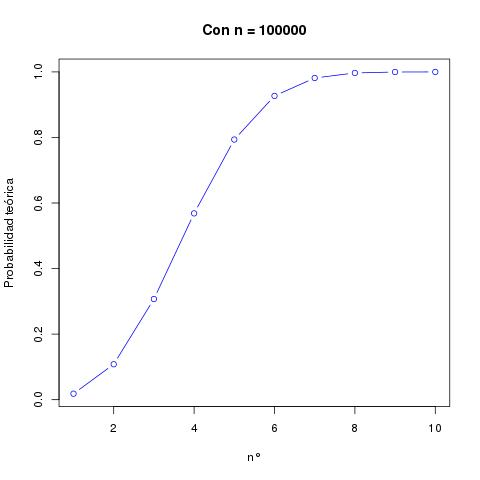
\includegraphics[width=\linewidth]{p4_teo_100000.jpg}
              \caption{P. Te\'orica para n = 100000}
          \end{figure}
      \end{minipage}
      \hspace{0.05\linewidth}
      \begin{minipage}{0.45\linewidth}
          \begin{figure}[H]
              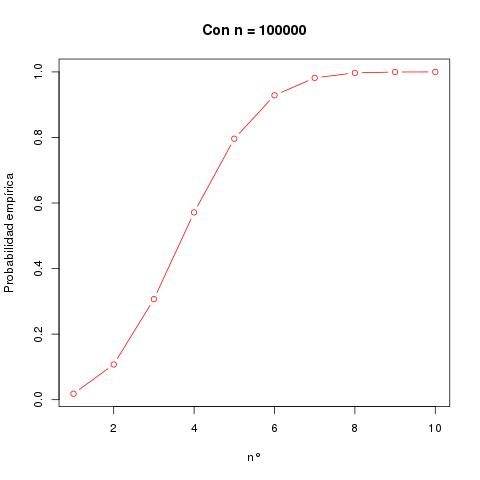
\includegraphics[width=\linewidth]{p4_emp_100000.jpg}
              \caption{P. Emp\'irica para n = 100000}
          \end{figure}
      \end{minipage}
  \end{minipage}
  
\item[b)]
Finalmente para un $n = 100000$ se encuentra una convergencia menor a 0.01, para el caso puntual
es de 0.008844152.
 
\end{itemize}

\subsection{Pregunta 5}

Al ser cauchy una distribución continua se tomarán valores por intervalos a los cuales se calculará la probabilidad
empírica y teórica respectivamente para distintos $n$ pedidos.
\begin{itemize}
 \item[a)] 
      Luego de varias muestras para obtenidas de la distribución, se grafica los errores desde el menor $n$ hasta el mayor, el como
      disminuye este error hasta llegara 0 (o casi 0) permite apreciar la convergencia de la probabilidad empírica hacia la teórica con pruebas
      de ello, mostrando que la gran cantidad de experimentos logra representar el fenómeno a estudiar. Se utilizan $n=10,20,30,40,50,100,200,300,400,500,1000,1500,2000,5000,10000,100000$.
     
      \begin{figure}[H]
	      \centering
              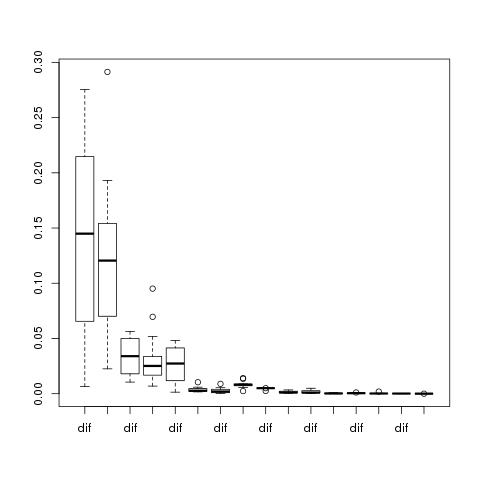
\includegraphics[width=100mm, scale=0.3]{p5a_boxplot_dif.jpg}
              \caption{Boxplot de error a medida que se aumenta el tamaño de la muestra}
          \end{figure}


      \begin{figure}[H]
        \centering
              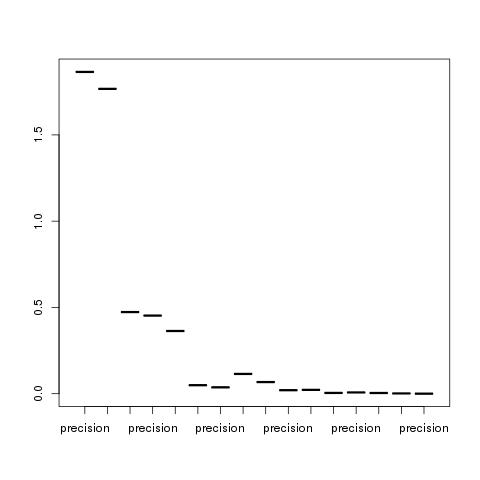
\includegraphics[width=100mm, scale=0.3]{p5a_boxplot_conv.jpg}
              \caption{Boxplot de error a medida que se aumenta el tamaño de la muestra}
          \end{figure}


\begin{table}[H]
    \centering
    \begin{tabular}{|l|l|}
    \hline
    $n$ & error \\ \hline
    $10    $  &    $1.865062  $\\
    $20    $  &    $1.766909 $\\
    $30    $  &    $0.4731489$   \\
    $40    $  &    $0.452522 $  \\
    $50    $  &    $0.3633154 $   \\
    $100   $  &    $0.04919491$    \\
    $200   $  &    $0.03697775$    \\
    $300   $  &    $0.1146243$    \\
    $400   $  &    $0.06749258$     \\
    $500   $  &    $0.02033396 $     \\
    $1000  $   &   $0.02223003$     \\
    $1500  $  &    $0.004464918 $   \\
    $2000  $  &    $0.007289842$    \\
    $5000  $  &    $0.004053419 $     \\
    $10000 $   &   $0.001490559$   \\
    $100000$   &   $1.380873e-05$   \\ \hline
    \end{tabular}
\end{table}
      



 \item[b)]
 
    Se matienen los valores de n, $n=10,20,30,40,50,100,200,300,400,500,1000,1500,2000,5000,10000,100000$. Con los cuales se calculan los errore respectivos que seŕan mostrados 
    con boxplots.
       \begin{figure}[H]
	      \centering
              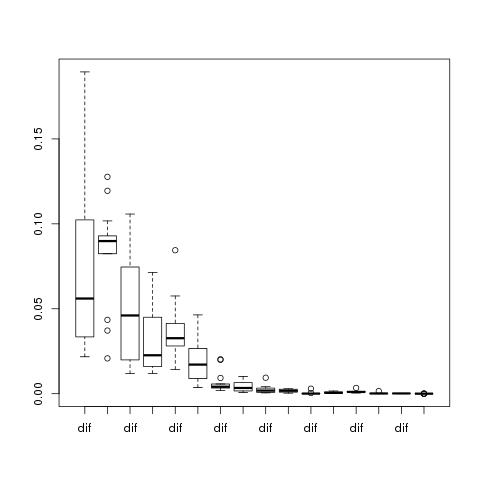
\includegraphics[width=100mm, scale=0.3]{p5b_boxplot_dif.jpg}
              \caption{Boxplot de error a medida que se aumenta el tamaño de la muestra, location 20, scale = 30}
          \end{figure}

       \begin{figure}[H]
        \centering
              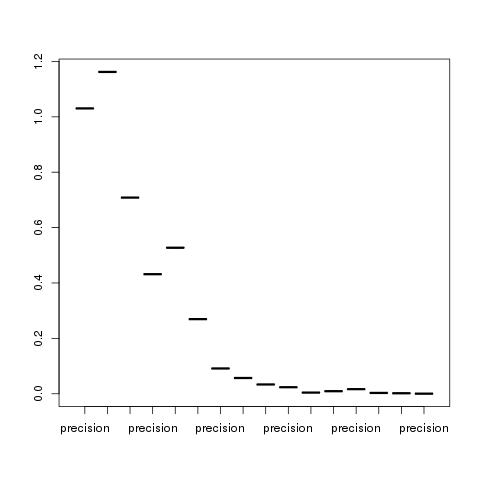
\includegraphics[width=100mm, scale=0.3]{p5b_boxplot_conv.jpg}
              \caption{Boxplot de error a medida que se aumenta el tamaño de la muestra, location 20, scale = 30}
          \end{figure}


\begin{table}[H]
    \centering
    \begin{tabular}{|l|l|}
    \hline
    $n$ & error \\ \hline
    10      &    1.030443  \\
    20      &    1.16216   \\
    30      &     0.7083201   \\
    40      &    0.4317799   \\
    50      &    0.5272908    \\
    100     &    0.2695098     \\
    200     &    0.09134366    \\
    300     &    0.05696333    \\
    400     &    0.03351027     \\
    500     &    0.02355948     \\
    1000     &   0.004144235     \\
    1500    &    0.009238539   \\
    2000    &    0.01659956    \\
    5000    &    0.003058157     \\
    10000    &    0.00183897   \\
    100000   &   0.0002454811   \\ \hline
    \end{tabular}
\end{table}


     precision precision precision precision precision precision  precision  precision
[1,]  1.030443   1.16216 0.7083201 0.4317799 0.5272908 0.2695098 0.09134366 0.05696333
      precision  precision   precision   precision  precision   precision  precision
[1,] 0.03351027 0.02355948 0.004144235 0.009238539 0.01659956 0.003058157 0.00183897
        precision
[1,] 0.0002454811
      
 
\end{itemize}

\subsection{Pregunta 6}

Como se ha hecho para el caso anterior, se tomaron intervalos para agrupar los datos y poder calcular
las frecuencias relativas, junto a ello obtener la probabilidad empírica y teórica. Los experimentos
realizados son para $n=10,20,30,40,50,100,200,300,400,500,1000,1500,2000,5000,10000,100000$ siendo estos un total de $16$. A cotinuación se muestra
el boxplot que refleja la convergencia de las probabilidades. 

       \begin{figure}[H]
	      \centering
              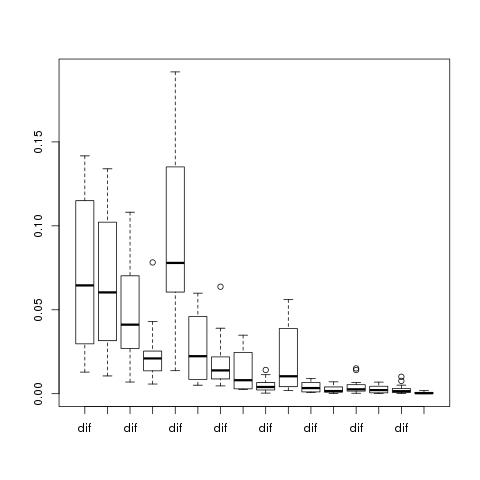
\includegraphics[width=100mm, scale=0.3]{p6_boxplot_dif.jpg}
              \caption{Boxplot de error a medida que se aumenta el tamaño de la muestra}
          \end{figure}

Para este caso se puede ver que que la convergencia no es tan estable hasta que se alcanza un $n=1000$, siendo el caso final.
Tarda más en converger respecto a los experimentos de preguntas anteriores. Gráficamente es lo siguiente

      \begin{figure}[H]
        \centering
              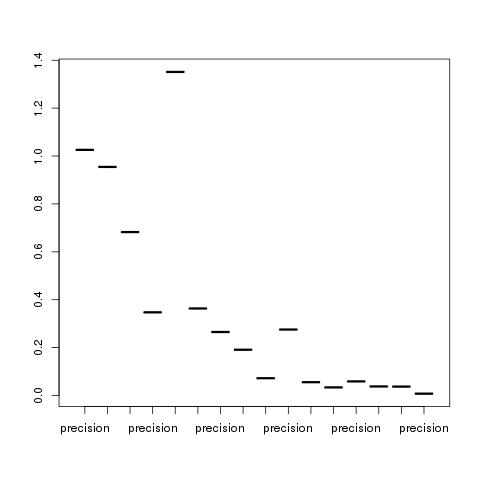
\includegraphics[width=100mm, scale=0.3]{p6_boxplot_conv.jpg}
              \caption{Boxplot de los errores puntuales a medida que se aumenta el tamaño de la muestra}
          \end{figure}

Donde la diferencia se obtiene para $n=100000$.

Para detallar lo anterior se construye una tabla para mostrar el error para cada $n$:

\begin{table}[H]
    \centering
    \begin{tabular}{|l|l|}
    \hline
    $n$ & error \\ \hline
    10      & 1.025721     \\
    20      & 0.9544134     \\
    30      & 0.6825494    \\
    40      & 0.3473851    \\
    50      & 1.351208    \\
    100     & 0.3634327     \\
    200     & 0.2651737    \\
    300     & 0.1910359     \\
    400     & 0.07210407     \\
    500     & 0.2754461     \\
    1000     & 0.05544603     \\
    1500    & 0.03382561    \\
    2000    & 0.05880897    \\
    5000    & 0.03764551     \\
    10000    & 0.03716417    \\
    100000   & 0.007556121   \\ \hline
    \end{tabular}
\end{table}

 

\newpage
\subsection{Pregunta 7}
El uso de la probabilidad empiríca es un estimador de la función de densidad de probabilidad. El teorema de Glivenko-Cantelli tiene aplicaciones
en esta área:
\begin{itemize}
    \item Estimación puntual de parámetros de posición.
    \item Estimación puntual de parámetros de robustez.
    \item Estimación por intervalos de parámetros. 

\end{itemize}




\section{Conclusiones}


%\section{Anexos}


%\bibliographystyle{alpha}
%\bibliography{bibbase}

% referencias
%[1] Nombre de la referencia, Autor.



\end{document}
